\chapter{Convolutional Neural Networks} \label{sec:chapterCNN}

\minitoc

\section{Introduction}

\yinipar{\fontsize{60pt}{72pt}\usefont{U}{Kramer}{xl}{n}I}n this chapter we review a second type of neural network that is presumably the most popular one: Convolutional Neural Networks (CNN). CNN are particularly adapted for image classification, be it numbers or animal/car/... category. We will review the novelty involved when dealing with CNN when compared to FNN. Among them are the fundamental building blocks of CNN: convolution and pooling. We will in addition see what modification have to be taken into account for the regularization techniques introduced in the FNN part. Finally, we will present the most common CNN architectures that are used in the literature: from LeNet to ResNet.


\section{CNN architecture}


A CNN is formed by several convolution and pooling operations, usually followed by one or more fully connected layers (those being similar to the traditional FNN layers). We will clarify the new terms introduced thus far in the following sections.


\begin{figure}[H]
\begin{center}
\begin{tikzpicture}
\node[] at (0,0) {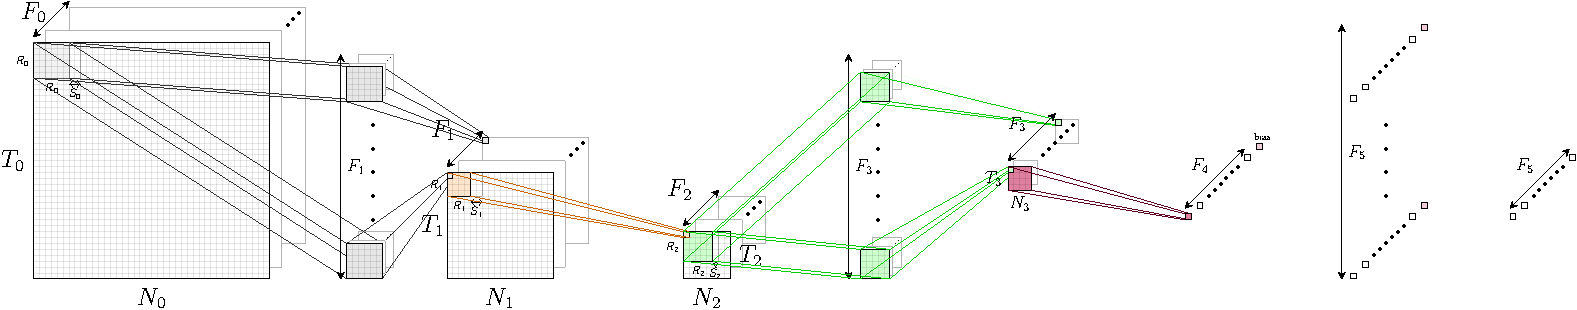
\includegraphics[scale=0.5]{CNN_MM_unpixels}};
\end{tikzpicture}
\caption{\label{fig:lenet-CNN}A typical CNN architecture (in this case LeNet inspired): convolution operations are followed by pooling operations, until the size of each feature map is reduced to one. Fully connected layers can then be introduced.}
\end{center}
\end{figure}

\section{CNN specificities}



\subsection{Feature map}

In each layer of a CNN, the data are no longer labeled by a single index as in a FNN. One should see the FNN index as equivalent to the label of a given image in a layer of a CNN. This label is the feature map. In each feature map $f\in \llbracket 0,F_\nu-1\rrbracket$ of the $\nu$'th layer, the image is fully characterized by two additional indices corresponding to its height $k\in T_\nu-1$ and its width $j\in N_\nu-1$. A given $f,j,k$ thus characterizes a unique pixel of a given feature map. Let us now review the different layers of a CNN

\subsection{Input layer}


We will be considering a input of $F_0$ channels. In the standard image treatment, these channels can correspond to the RGB colors ($F_0=3$). Each image in each channel will be of size $N_0\times T_0$ (width$\times$height). The input will be denoted $X^{(t)}_{f\,j\,k}$, with $t\in \llbracket 0, T_{{\rm mb}}-1\rrbracket$ (size of the Mini-batch set, see chapter \ref{sec:chapterFNN}), $j \in \llbracket 0, N_0-1\rrbracket$ and $k \in \llbracket 0, T_0-1\rrbracket$. A standard input treatment is to center the data following either one of the two following procedure
\begin{align}
\tilde{X}^{(t)}_{f\,j\,k}&=X^{(t)}_{i\,j\,k}-\mu_{f}\;,&
%
\tilde{X}^{(t)}_{f\,j\,k}&=X^{(t)}_{i\,j\,k}-\mu_{f\,j\,k}\;
\end{align}
with
\begin{align}
\mu_{f}&=\frac{1}{T_{{\rm train}}T_0 N_0}\sum^{T_{{\rm train}}-1}_{t=0}\sum_j^{N_0-1}
%
\sum_k^{T_0-1}X^{(t)}_{f\,j\,k}\;,\\
%
\mu_{f\,j\,k}&=\frac{1}{T_{{\rm train}}}\sum^{T_{{\rm train}}-1}_{t=0}X^{(t)}_{f\,j\,k}\;.
\end{align}
This correspond to either compute the mean per pixel over the training set, or to also average over every pixel. This procedure should not be followed for regression tasks. To conclude, figure \ref{fig:input_layer} shows what the input layer looks like.

\begin{figure}[H]
\begin{center}
\begin{tikzpicture}
\node[] at (0,0) {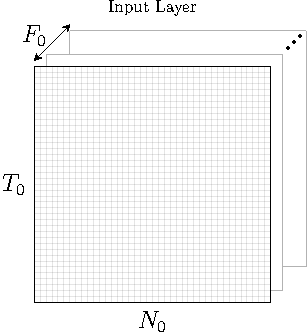
\includegraphics[scale=1]{input_layer}};
\end{tikzpicture}
\caption{\label{fig:input_layer} The Input layer}
\end{center}
\end{figure}

\subsection{Padding}

As we will see when we proceed, it may be convenient to "pad" the feature maps in order to preserve the width and the height of the images though several hidden layers. The padding operation amounts to add $0$'s around the original image. With a padding of size $P$, we add $P$ zeros at the beginning of each row and column of a given feature map. This is illustrated in the following figure

\begin{figure}[H]
\begin{center}
\begin{tikzpicture}
\node[] at (0,0) {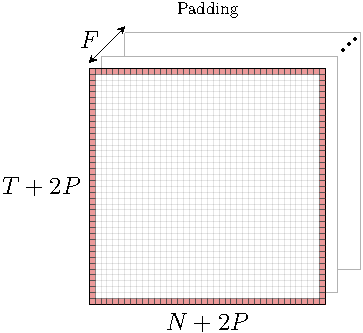
\includegraphics[scale=1]{padding}};
\end{tikzpicture}
\caption{Padding of the feature maps. The zeros added correspond to the red tiles, hence a padding of size $P=1$.}
\end{center}
\end{figure}

\subsection{Convolution}

The convolution operation that gives its name to the CNN is the fundamental building block of this type of network. It amounts to convolute a feature map of an input hidden layer with a weight matrix to give rise to an output feature map. The weight is really a four dimensional tensor, one dimension ($F$) being the number of feature maps of the convolutional input layer, another ($F_p$) the number of feature maps of the convolutional output layer. The two others gives the size of the receptive field in the width and the height direction. The receptive field allows one to convolute a subset instead of the whole input image. It aims at searching similar patterns in the input image, no matter where the pattern is (translational invariance). The width and the height of the output image are also determined by the stride: it is simply the number of pixel by which one slides in the vertical and/or the horizontal direction before applying again the convolution operation. A good picture being worth a thousand words, here is the convolution operation in a nutshell

\begin{figure}[H]
\begin{center}
\begin{tikzpicture}
\node[] at (0,0) {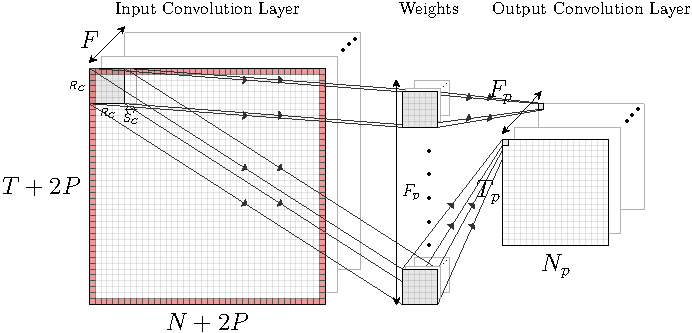
\includegraphics[scale=1]{VGG-conv}};
\end{tikzpicture}
\caption{The convolution operation}
\end{center}
\end{figure}

Here $R_C$ is the size of the convolutional receptive field (we will see that the pooling operation also has a receptive field and a stride) and $S_C$ the convolutional stride. The widths and heights of the output image can be computed thanks to the input height $T$ and output width $N$
\begin{align}
N_p&=\frac{N+2P-R_C}{S_C}+1 \;,&
%
T_p&=\frac{T+2P-R_C}{S_C}+1\;.
\end{align}
It is common to introduce a padding to preserve the widths and heights of the input image $N=N_p=T=T_p$, so that in these cases $S_C=1$ and
\begin{align}
P&=\frac{R_C-1}{2}\;.
\end{align}
For a given layer $n$, the convolution operation mathematically reads (similar in spirit to the weight averaging procedure of a FNN)
\begin{align}
a_{f\,l\,m}^{(t)(\nu)}&=\sum^{F_\nu-1}_{\nu=0}\sum^{R_C-1}_{j=0}\sum^{R_C-1}_{k=0}
%
\Theta^{(o)f}_{f\,j\,k}h^{(t)(\nu)}_{f\,S_Cl+j\,S_Cm+k}\;,
\end{align}
where $o$ characterizes the $o+1$ convolution in the network. Here $\nu$ denotes the $\nu$'th hidden layer of the network (and thus belongs to $\llbracket0,N-1 \rrbracket$), and $f\in\llbracket0,F_{\nu+1}-1\rrbracket$, $l\in\llbracket0,N_{\nu+1}-1 \rrbracket$ and $m\in\llbracket0,T_{\nu+1}-1 \rrbracket$. Thus $S_Cl+j\in\llbracket0,N_\nu-1 \rrbracket$ and $S_Cl+j\in\llbracket0,T_\nu-1 \rrbracket$. One then obtains the hidden units via a ReLU (or other, see chapter \ref{sec:chapterFNN}) activation function application. Taking padding into account, it reads
\begin{align}
h_{f\,l+P\,m+P}^{(t)(\nu+1)}&=g\left(a_{f\,l\,m}^{(t)(\nu)}\right)\;.
\end{align} 


\subsection{Pooling}

The pooling operation, less and less used in the current state of the art CNN, is fundamentally a dimension reduction operation. It amounts either to average or to take the maximum of a sub-image -- characterized by a pooling receptive field $R_P$ and a stride $S_P$ -- of the input feature map $F$ to obtain an output feature map $F_p=F$ of width $N_p<N$ and height $T_p<T$. To be noted: the padded values of the input hidden layers are not taken into account during the pooling operation (hence the $+P$ indices in the following formulas)


\begin{figure}[H]
\begin{center}
\begin{tikzpicture}
\node[] at (0,0) {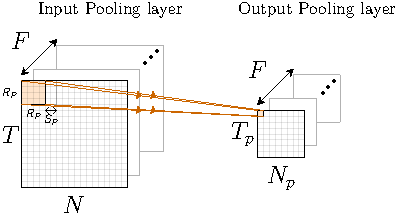
\includegraphics[scale=1]{VGG-pool}};
\end{tikzpicture}
\caption{The pooling operation}
\end{center}
\end{figure}

The average pooling procedure reads for a given $\nu$'th pooling operation
\begin{align}
a_{f\,l\,m}^{(t)(\nu)}&=\sum^{R_P-1}_{j,k=0} h_{f\,S_P l+j+P\,S_Pm+k+P}^{(t)(\nu)}\;,
\end{align}
while the max pooling reads
\begin{align}
a_{f\,l\,m}^{(t)(\nu)}&=\max^{R_P-1}_{j,k=0} h_{f\,S_P l+j+P\,S_Pm+k+P}^{(t)(\nu)}\;.
\end{align}
Here $\nu$ denotes the $\nu$'th hidden layer of the network (and thus belongs to $\llbracket0,N-1 \rrbracket$), and $f\in\llbracket0,F_{\nu+1}-1\rrbracket$, $l\in\llbracket0,N_{\nu+1}-1 \rrbracket$ and $m\in\llbracket0,T_{\nu+1}-1 \rrbracket$. Thus $S_Pl+j\in\llbracket0,N_\nu-1 \rrbracket$ and $S_Pl+j\in\llbracket0,T_\nu-1 \rrbracket$. Max pooling is extensively used in the literature, and we will therefore adopt it in all the following. Denoting $j^{(t)(p)}_{_{flm}},\,k^{(t)(p)}_{_{flm}}$ the indices at which the $l,m$ maximum  of the $f$ feature map of the $t$'th batch sample is reached, we have
\begin{align}
h_{f\,l+P\,m+P}^{(t)(\nu+1)}&=a_{f\,l\,m}^{(t)(\nu)}=
%
h^{(t)(\nu)}_{f\,S_P l+j^{(t)(p)}_{_{flm}}+P\,S_Pm+k^{(t)(p)}_{_{flm}}+P}\;.
\end{align}

\subsection{Towards fully connected layers}

At some point in a CNN the convolutional receptive field is equal to the width and the height of the input image. In this case, the convolution operation becomes a kind of weight averaging procedure (as in a FNN)


\begin{figure}[H]
\begin{center}
\begin{tikzpicture}
\node[] at (0,0) {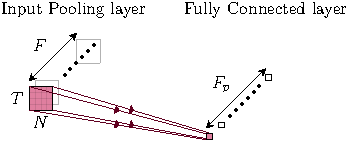
\includegraphics[scale=1]{VGG-pool-fc}};
\end{tikzpicture}
\caption{Fully connected operation to get images of width and height $1$.}
\end{center}
\end{figure}

This weight averaging procedure reads
\begin{align}
a_{f}^{(t)(\nu)}&=\sum^{F_\nu-1}_{f'=0}\sum^{N-1}_{l=0}
%
\sum^{T-1}_{m=0}\Theta^{(o)f}_{f'lm}h^{(t)(\nu)}_{f'l+Pm+P}\;,
\end{align}
and is followed by the activation function
\begin{align}
h_{f}^{(t)(\nu+1)}&=g\left(a_{f}^{(t)(\nu)}\right)\;,
\end{align}
\subsection{fully connected layers}

After the previous operation, the remaining network is just a FNN one. The weigh averaging procedure reads

\begin{align}
a_{f}^{(t)(\nu)}&=\sum^{F_\nu-1}_{f'=0}\Theta^{(o)f}_{f'}h^{(t)(\nu)}_{f'}\;,
\end{align}
and is followed as usual by the activation function
 \begin{align}
h_{f}^{(t)(\nu+1)}&=g\left(a_{f}^{(t)(\nu)}\right)\;,
\end{align}

\begin{figure}[H]
\begin{center}
\begin{tikzpicture}
\node[] at (0,0) {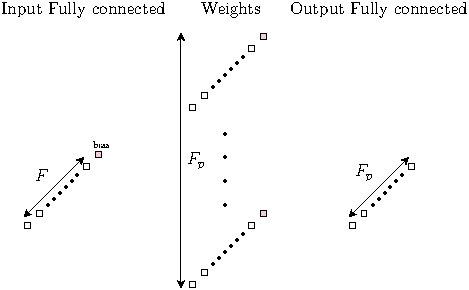
\includegraphics[scale=1]{VGG-fc}};
\end{tikzpicture}
\caption{Fully connected operation, identical to the FNN operations.}
\end{center}
\end{figure}

\subsection{Output connected layer}

Finally, the output is computed as in a FNN
\begin{align}
a_{f}^{(t)(N-1)}&=\sum^{F_{N}-1}_{f'=0}\Theta^{(o)f}_{f'}h^{(t)(N-1)}_{f'}\;,
&
h_{f}^{(t)(N)}&=o\left(a_{f}^{(t)(N-1)}\right)\;,
\end{align}
where as in a FNN, $o$ is either the L2 or the cross-entropy loss function (see chapter \ref{sec:chapterFNN}). 

\section{Modification to Batch Normalization}


In a CNN, Batch normalization is modified in the following way (here, contrary to a regular FNN, not all the hidden layers need to be Batch normalized. Indeed this operation is not performed on the output of the pooling layers. We will hence use different names $\nu$ and $n$ for the regular and batch normalized hidden layers) 
\begin{align}
\tilde{h}_{f\,l\,m}^{(t)(n)}&=\frac{h_{f\,l\,m}^{(t)(\nu)}-\hat{h}_{f}^{(n)}}
%
{\sqrt{\left(\hat{\sigma}_{f}^{(n)}\right)^2+\epsilon}}\;,
\end{align}
with
\begin{align}
\hat{h}_{f}^{(n)}&=
%
\frac{1}{T_{{\rm mb}}N_nT_n}\sum^{T_{{\rm mb}}-1}_{t=0}\sum^{N_n-1}_{l=0}\sum^{T_n-1}_{m=0}h_{f\,l\,m}^{(t)(\nu)}\\
%
\left(\hat{\sigma}_{f}^{(n)}\right)^2&=\frac{1}{T_{{\rm mb}}N_nT_n}\sum^{T_{{\rm mb}}-1}_{t=0}
%
\sum^{N_n-1}_{l=0}\sum^{T_n-1}_{m=0}\left(h_{f\,l\,m}^{(t)(\nu)}-\hat{h}_{f}^{(n)}\right)^2\;.
\end{align}
The identity transform can be implemented thanks to the two additional parameters $(\gamma_f,\beta_f)$ 
\begin{align}
y^{(t)(n)}_{f\,l\,m}&=\gamma^{(n)}_f\,\tilde{h}_{f\,l\,m}^{(t)(n)}+\beta^{(n)}_f\;.
\end{align}
For the evaluation of the cross-validation and the test set (calling e the number of iterations/epochs), one has to compute
\begin{align}
\mathbb{E}\left[h_{f\,l\,m}^{(t)(\nu)}\right]_{e+1} &=
%
\frac{e\mathbb{E}\left[h_{f\,l\,m}^{(t)(\nu)}\right]_{e}+\hat{h}_{f}^{(n)}}{e+1}\;,\\
%
\mathbb{V}ar\left[h_{f\,l\,m}^{(t)(\nu)}\right]_{e+1} &=
%
\frac{i\mathbb{V}ar\left[h_{f\,l\,m}^{(t)(\nu)}\right]_{e}+\left(\hat{\sigma}_{f}^{(n)}\right)^2}{e+1}
\end{align}
and what will be used at test time is $\mathbb{E}\left[h_{f\,l\,m}^{(t)(\nu)}\right]$ and $\frac{T_{{\rm mb}}}{T_{{\rm mb}}-1}\mathbb{V}ar\left[h_{f\,l\,m}^{(t)(\nu)}\right]$.


\section{Network architectures}

We will now review the standard CNN architectures that have been used in the literature in the past 20 years, from old to very recent (end of 2015) ones. To allow for an easy graphical representation, we will adopt the following schematic representation of the different layers.

\begin{figure}[H]
\begin{align*}
\begin{tikzpicture}[baseline=-3pt]
\node[] at (0,0) {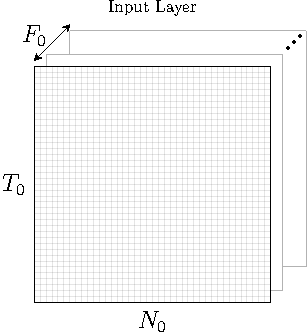
\includegraphics[scale=0.5]{input_layer}};
\end{tikzpicture}&=
%
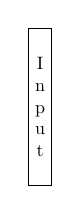
\begin{tikzpicture}[baseline=-0pt]
\draw (0,-1) rectangle (0+0.3,1); 
\node[align=center,scale = 0.65] at (0+0.15,0) {I \\ n \\ p \\ u \\ t};
\end{tikzpicture}\;,&
%
\begin{tikzpicture}[baseline=-3pt]
\node[] at (0,0) {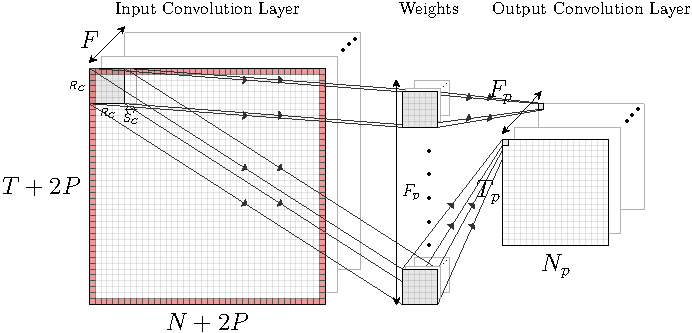
\includegraphics[scale=0.5]{VGG-conv}};
\end{tikzpicture}&=
%
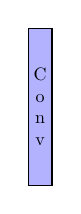
\begin{tikzpicture}[baseline=-0pt]
\filldraw[fill=blue!30!white] (0,-1) rectangle (0+0.3,1); 
\node[align=center,scale = 0.65] at (0+0.15,0) {C \\ o \\ n \\ v};
\end{tikzpicture}\;,\notag\\
%
\begin{tikzpicture}[baseline=-3pt]
\node[] at (0,0) {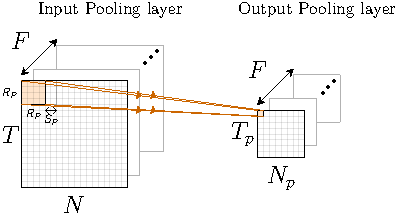
\includegraphics[scale=0.5]{VGG-pool}};
\end{tikzpicture}&=
%
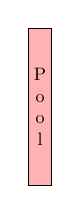
\begin{tikzpicture}[baseline=-0pt]
\filldraw[fill=red!30!white] (0,-1) rectangle (0+0.3,1); 
\node[align=center,scale = 0.65] at (0+0.15,0) {P \\ o \\ o \\ l};
\end{tikzpicture}\;,&
%
\begin{tikzpicture}[baseline=-3pt]
\node[] at (0,0) {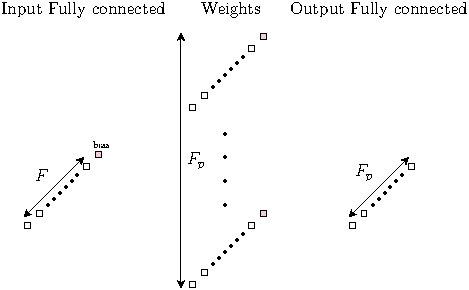
\includegraphics[scale=0.5]{VGG-fc}};
\end{tikzpicture}&=
%
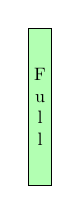
\begin{tikzpicture}[baseline=-0pt]
\filldraw[fill=green!30!white] (0,-1) rectangle (0+0.3,1); 
\node[align=center,scale = 0.65] at (0+0.15,0) {F \\ u \\ l \\ l};
\end{tikzpicture}
\end{align*}
\begin{center}
\caption{Schematic representation of the different layer}
\end{center}
\end{figure}


\subsection{Realistic architectures}

In realistic architectures, every fully connected layer (except the last one related to the output) is followed by a ReLU (or other) activation and then a batch normalization step (these two data processing steps can be inverted, as it was the case in the original BN implementation).
\begin{figure}[H]
\begin{center}
\begin{tikzpicture}
\node[] at (0,0) {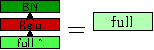
\includegraphics[scale=1.5]{fc_equiv}};
\end{tikzpicture}
\caption{Realistic Fully connected operation}
\end{center}
\end{figure}
 The same holds for convolutional layers
\begin{figure}[H]
\begin{center}
\begin{tikzpicture}
\node[] at (0,0) {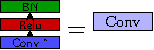
\includegraphics[scale=1.5]{Conv_equiv}};
\end{tikzpicture}
\caption{Realistic Convolution operation}
\end{center}
\end{figure}

We will adopt the simplified right hand side representation, keeping in mind that the true structure of a CNN is richer. With this in mind -- and mentioning in passing \cite{Gu2015RecentAI} that details recent CNN advances, let us now turn to the first popular CNN used by the deep learning community.

\subsection{LeNet}

The LeNet\cite{Lecun98gradient-basedlearning} (end of the 90's) network is formed by an input, followed by two conv-pool layers and then a fully-connected layer before the final output. It can be seen in figure \ref{fig:lenet-CNN} 
\begin{figure}[H]
\begin{center}
\begin{tikzpicture}
\node[] at (0,0) {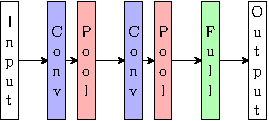
\includegraphics[scale=1]{LeNet}};
\end{tikzpicture}
\caption{The LeNet CNN}
\end{center}
\end{figure}

When treating large images ($224\times 224$), this implies to use large size of receptive fields and strides. This has two downsides. Firstly, the number or parameter in a given weight matrix is proportional to the size of the receptive field, hence the larger it is the larger the number of parameter. The network can thus be more prone to overfit. Second, a large stride and receptive field means a less subtle analysis of the fine structures of the images. All the subsequent CNN implementations aim at reducing one of these two issues.

\subsection{AlexNet}

The AlexNet\cite{NIPS2012_4824} (2012) saw no qualitative leap in the CNN theory, but due to better processors was able to deal with more hidden layers.

\begin{figure}[H]
\begin{center}
\begin{tikzpicture}
\node[] at (0,0) {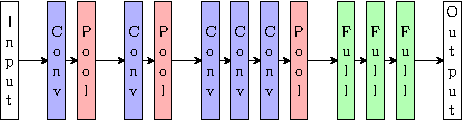
\includegraphics[scale=1]{AlexNet}};
\end{tikzpicture}
\caption{The AlexNet CNN}
\end{center}
\end{figure}

This network is still commonly used, though less since the arrival of the VGG network.

\subsection{VGG}

The VGG\cite{DBLP:journals/corr/SimonyanZ14a} network (2014) adopted a simple criteria: only $2 \times 2$ paddings of stride $2$ and $3\times 3$ convolutions of stride $1$ with a padding of size $1$, hence preserving the size of the image's width and height through the convolution operations.

\begin{figure}[H]
\begin{center}
\begin{tikzpicture}
\node[] at (0,0) {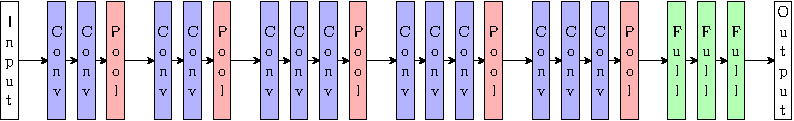
\includegraphics[scale=1]{VGG}};
\end{tikzpicture}
\caption{The VGG CNN}
\end{center}
\end{figure}

This network is the standard one in most of the deep learning packages dealing with CNN. It is no longer the state of the art though, as a design innovation has taken place since its creation. 

\subsection{GoogleNet}

The GoogleNet\cite{43022} introduced a new type of "layer" (which is in reality a combination of existing layers): the inception layer (in reference to the movie by Christopher Nolan). Instead of passing from one layer of a CNN to the next by a simple pool, conv or fully-connected (fc) operation, one averages the result of the following architecture.

\begin{figure}[H]
\begin{center}
\begin{tikzpicture}
\node[] at (0,0) {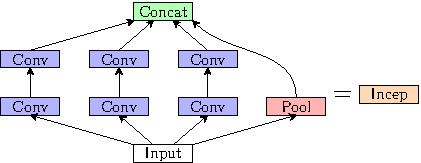
\includegraphics[scale=1]{Inception}};
\end{tikzpicture}
\caption{The Inception module}
\end{center}
\end{figure}

We won't enter into the details of the concat layer, as the Google Net illustrated on the following figure is (already!) no longer state of the art.


\begin{figure}[H]
\begin{center}
\begin{tikzpicture}
\node[] at (0,0) {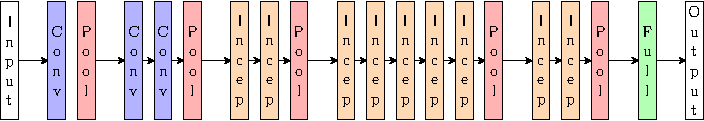
\includegraphics[scale=1]{GoogleNet}};
\end{tikzpicture}
\caption{The GoogleNet CNN}
\end{center}
\end{figure}

Indeed, the idea of averaging the result of several conv-pool operations to obtain the next hidden layer of a CNN as been exploited but greatly simplified by the state of the art CNN : The ResNet.

\subsection{ResNet}

\begin{figure}[H]
\begin{center}
\begin{align*}
&\begin{tikzpicture}
\node[] at (0,0) {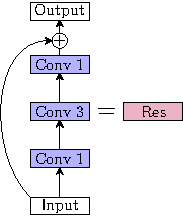
\includegraphics[scale=1.3]{Bottleneck}};
\end{tikzpicture}&
%
\begin{tikzpicture}
\node[] at (0,0) {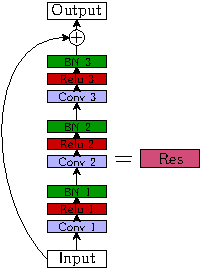
\includegraphics[scale=1]{Bottleneck_BN}};
\end{tikzpicture}
\end{align*}
\caption{\label{fig:Bottleneck_BN}The Bottleneck Residual architecture. Schematic representation on the left, realistic one on the right. It amounts to a $1\times 1$ conv of stride $1$ and padding $0$, then a standard VGG conv and again a $1 \times 1$ conv. Two main modifications in our presentation of ResNet: BN operations have been put after ReLU ones, and the final ReLU is before the plus operation.}
\end{center}
\end{figure}

The ResNet\cite{He2015} takes back the simple idea of the VGG net to always use the same size for the convolution operations (except for the first one). It also takes into account an experimental fact: the fully connected layer (that usually contains most of the parameters given their size) are not really necessary to perform well. Removing them leads to a great decrease of the number of parameters of a CNN. In addition, the pooling operation is also less and less popular and tend to be replaced by convolution operations. This gives the basic ingredients of the ResNet fundamental building block, the Residual module of figure \ref{fig:Bottleneck_BN}.

\vspace{0.2cm}

Two important points have to be mentioned concerning the Residual module. Firstly, a usual conv-conv-conv structure would lead to the following output (forgetting about batch normalization for simplicity and only for the time being, and denoting that there is no need for padding in $1\times 1$ convolution operations)
\begin{align}
h^{(t)(1)}_{fl+Pm+P}&=
%
g\left(\sum^{F_0-1}_{f'=0}\sum^{R_C-1}_{j=0}\sum^{R_C-1}_{k=0}
%
\Theta^{(0)f}_{f'\,j\,k}h^{(t)(0)}_{f'\,S_Cl+j\,S_Cm+k}\right)\notag\\
%
h^{(t)(2)}_{flm}&=
%
g\left(\sum^{F_1-1}_{f'=0}\sum^{R_C-1}_{j=0}\sum^{R_C-1}_{k=0}
%
\Theta^{(0)f}_{f'\,j\,k}h^{(t)(1)}_{f'\,S_Cl+j\,S_Cm+k}\right)\notag\\
%
h^{(t)(3)}_{flm}&=
%
g\left(\sum^{F_2-1}_{f'=0}\sum^{R_C-1}_{j=0}\sum^{R_C-1}_{k=0}
%
\Theta^{(0)f}_{f'\,j\,k}h^{(t)(2)}_{f'\,S_Cl+j\,S_Cm+k}\right)\;,
\end{align}
whereas the Residual module modifies the last previous equation to (implying that the width, the size and the number of feature size of the input and the output being the same)
\begin{align}
h^{(t)(4)}_{flm}&=h^{(t)(0)}_{flm}+g\left(
%
\sum^{F_2-1}_{f'=0}\sum^{R_C-1}_{j=0}\sum^{R_C-1}_{k=0}
%
\Theta^{(0)f}_{f'\,j\,k}h^{(t)(2)}_{f'\,S_Cl+j\,S_Cm+k}\right)\notag\\
%
&=h^{(t)(0)}_{flm}+\delta h^{(t)(0)}_{flm}\;.
\end{align}
Instead of trying to fit the input, one is trying to fit a tiny modification of the input, hence the name residual. This allows the network to minimally modify the input when necessary, contrary to traditional architectures. Secondly, if the number of feature maps is important, a $3\times 3$ convolution with stride 1 could be very costly in term of execution time and prone to overfit (large number of parameters). This is the reason of the presence of the $1 \times 1$ convolution, whose aim is just to prepare the input to the $3\times 3$ conv to reduce the number of feature maps, number which is then restored with the final $1\times 1$ conv of the Residual module. The first $1\times 1$ convolution thus reads as a weight averaging operation 
\begin{align}
h^{(t)(1)}_{fl+Pm+P}&=
%
g\left(\sum^{F_0-1}_{f'=0}
%
\Theta^{(0)f}_{f'}h^{(t)(0)}_{f'\,l\,m}\right)\;,
\end{align}
but is designed such that $f\in F_1\ll F_0$. The second $1\times 1$ convolution reads
\begin{align}
h^{(t)(3)}_{flm}&=g\left(\sum^{F_1-1}_{i=0}\Theta^{(2)f}_{i}h^{(t)(1)}_{i\,l\,m}\right)\;,
\end{align}
with $f \in F_0$, restoring the initial feature map size. The ResNet architecture is then the stacking of a large number (usually 50) of Residual modules, preceded by a conv-pool layer and ended by a pooling operation to obtain a fully connected layer, to which the output function is directly applied. This is illustrated in the following figure.



\begin{figure}[H]
\begin{center}
\begin{tikzpicture}
\node[] at (0,0) {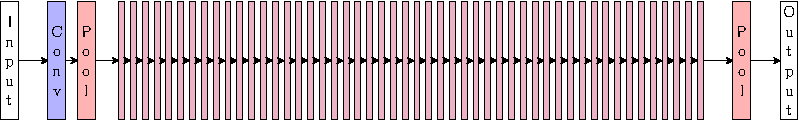
\includegraphics[scale=1]{ResNet}};
\end{tikzpicture}
\caption{The ResNet CNN}
\end{center}
\end{figure}


The ResNet CNN has accomplished state of the art results on a number of popular training sets (CIFAR, MNIST...). In practice, we will present in the following the backpropagation algorithm for CNN having standard (like VGG) architectures in mind.

\section{Backpropagation}

In a FNN, one just has to compute two kind of backpropagations : from output to fully connected (fc) layer and from fc to fc. In a traditional CNN, 4 new kind of propagations have to be computed: fc to pool, pool to conv, conv to conv and conv to pool. We present the corresponding error rates in the next sections, postponing their derivation to the appendix. We will consider as in a FNN a network with an input layer labelled $0$, N-1 hidden layers labelled $i$ and an output layer labelled $N$ ($N+1$ layers in total in the network).


\subsection{Backpropagate through Batch Normalization} \label{sec:BackpropbatchnormCNN}

As in FNN, backpropagation introduces a new gradient 
\begin{align}
\delta^f_{f'}J^{(tt')(n)}_{fll'mm'}&=
%
\frac{\partial y^{(t')(n)}_{f'\,l'\,m'}}{\partial h_{f\,l\,m}^{(t)(\nu)}}\;.
\end{align}
we show in appendix \ref{sec:appenbatchnorm-vgg} that for pool and conv layers
\begin{align}
J^{(tt')(n)}_{fll'mm'}&=\tilde{\gamma}^{(n)}_f \left[\delta^{t'}_t\delta^{l'}_l\delta^{m'}_m-
%
\frac{1+\tilde{h}_{f\,l'\,m'}^{(t')(n)}\tilde{h}_{f\,l\,m}^{(t)(n)}}{T_{{\rm mb}}N_nT_n}\right]\;,
\end{align}
while we find the FNN result as expected for fc layers 
\begin{align}
J^{(tt')(n)}_{f}&=\tilde{\gamma}^{(n)}_f \left[\delta^{t'}_t-
%
\frac{1+\tilde{h}_{f}^{(t')(n)}\tilde{h}_{f}^{(t)(n)}}{T_{{\rm mb}}}\right]\;.
\end{align}

\subsection{Error updates}

We will call the specific CNN error rates (depending on whether we need padding or not)
\begin{align}
\delta^{(t)(\nu)}_{fl(+P)m(+P)}&=\frac{\partial }{\partial a_{f\,l\,m}^{(t)(i)}}J(\Theta)\;,
\end{align}


\subsubsection{Backpropagate from output to fc}

Backpropagate from output to fc is schematically illustrated on the following plot

\begin{figure}[H]
\begin{center}
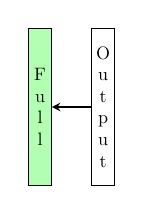
\begin{tikzpicture}[baseline=-0pt]
\draw (0.8,-1) rectangle (0.8+0.3,1); 
\node[align=center,scale = 0.65] at (0.8+0.15,0) {O \\ u \\ t \\ p \\ u \\ t};
\draw[-stealth]  (0.8,0) -- (0+0.3,0);
\filldraw[fill=green!30!white] (0,-1) rectangle (0+0.3,1); 
\node[align=center,scale = 0.65] at (0+0.15,0) {F \\ u \\ l \\ l};
\end{tikzpicture}
\caption{Backpropagate from output to fc.}
\end{center}
\end{figure}
As in FNN, we find for the L2 loss function
\begin{align}
\delta^{(t)(N-1)}_f&= \frac{1}{T_{{\rm mb}}}\left(h_{f}^{(t)(N)}-y_f^{(t)}\right)\;,
\end{align}
and for the cross-entropy one
\begin{align}
\delta^{(t)(N-1)}_f&= \frac{1}{T_{{\rm mb}}}\left(h_{f}^{(t)(N)}-\delta_{y^{(t)}}^f\right)\;,
\end{align}

\subsubsection{Backpropagate from fc to fc}

Backpropagate from fc to fc is schematically illustrated on the following plot

\begin{figure}[H]
\begin{center}
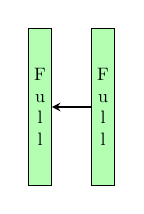
\begin{tikzpicture}[baseline=-0pt]
\filldraw[fill=green!30!white] (0.8,-1) rectangle (0.8+0.3,1); 
\node[align=center,scale = 0.65] at (0.8+0.15,0) {F \\ u \\ l \\ l};
\draw[-stealth]  (0.8,0) -- (0+0.3,0);
\filldraw[fill=green!30!white] (0,-1) rectangle (0+0.3,1); 
\node[align=center,scale = 0.65] at (0+0.15,0) {F \\ u \\ l \\ l};
\end{tikzpicture}
\caption{Backpropagate from fc to fc.}
\end{center}
\end{figure}
As in FNN, we find
\begin{align}
\delta^{(t)(\nu)}_f &=g'\left(a_{f}^{(t)(\nu)}\right)
%
\sum_{t'=0}^{T_{{\rm mb}}-1}\sum_{f'=0}^{F_{\nu+1}-1}\Theta^{(o)f'}_{f}J^{(tt')(n)}_{f} \delta^{(t)(\nu+1)}_{f'}\;,
\end{align}

\subsubsection{Backpropagate from fc to pool}

Backpropagate from fc to pool is schematically illustrated on the following plot

\begin{figure}[H]
\begin{center}
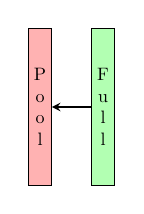
\begin{tikzpicture}[baseline=-0pt]
\filldraw[fill=green!30!white] (0.8,-1) rectangle (0.8+0.3,1); 
\node[align=center,scale = 0.65] at (0.8+0.15,0) {F \\ u \\ l \\ l};
\draw[-stealth]  (0.8,0) -- (0+0.3,0);
\filldraw[fill=red!30!white] (0,-1) rectangle (0+0.3,1); 
\node[align=center,scale = 0.65] at (0+0.15,0) {P \\ o \\ o \\ l};
\end{tikzpicture}
\caption{Backpropagate from fc to pool.}
\end{center}
\end{figure}
We show in appendix \ref{sec:appenderrorrate} that this induces the following error rate
\begin{align}
\delta^{(t)(\nu)}_{flm}&=\sum_{f'=0}^{F_{\nu+1}-1}\Theta^{(o)f'}_{f\,l\,m} \delta^{(t)(\nu+1)}_{f'}\;,
\end{align}

\subsubsection{Backpropagate from pool to conv}

Backpropagate from pool to conv is schematically illustrated on the following plot

\begin{figure}[H]
\begin{center}
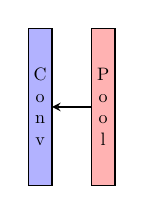
\begin{tikzpicture}[baseline=-0pt]
\filldraw[fill=red!30!white] (0.8,-1) rectangle (0.8+0.3,1); 
\node[align=center,scale = 0.65] at (0.8+0.15,0) {P \\ o \\ o \\ l};
\draw[-stealth]  (0.8,0) -- (0+0.3,0);
\filldraw[fill=blue!30!white] (0,-1) rectangle (0+0.3,1); 
\node[align=center,scale = 0.65] at (0+0.15,0) {C \\ o \\ n \\ v};
\end{tikzpicture}
\caption{Backpropagate from pool to conv.}
\end{center}
\end{figure}
We show in appendix \ref{sec:appenbatchnorm-vgg} that this induces the following error rate (calling the pooling layer the $p$th one)
\begin{align}
\delta^{(t)(\nu)}_{fl+Pm+P}&=g'\left(a_{f\,l\,m}^{(t)(\nu)}\right)
%
\sum_{t'=0}^{T_{{\rm mb}}-1}\sum^{N_{\nu+1}-1}_{l'=0}\sum^{T_{\nu+1}-1}_{m'=0}\delta_{fl'm'}^{(t')(\nu+1)}\notag\\
%
&\times J^{(tt')(n)}_{f\,S_P l'+j_{fl'm'}^{(t')(p)}+P\,S_Pm'+k_{fl'm'}^{(t')(p)}+P\,l+P\,m+P}\;.
\end{align}
Note that we have padded this error rate.

\subsubsection{Backpropagate from conv to conv}

Backpropagate from conv to conv is schematically illustrated on the following plot

\begin{figure}[H]
\begin{center}
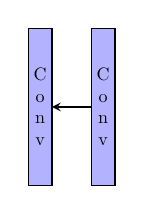
\begin{tikzpicture}[baseline=-0pt]
\filldraw[fill=blue!30!white] (0.8,-1) rectangle (0.8+0.3,1); 
\node[align=center,scale = 0.65] at (0.8+0.15,0)  {C \\ o \\ n \\ v};
\draw[-stealth]  (0.8,0) -- (0+0.3,0);
\filldraw[fill=blue!30!white] (0,-1) rectangle (0+0.3,1); 
\node[align=center,scale = 0.65] at (0+0.15,0) {C \\ o \\ n \\ v};
\end{tikzpicture}
\caption{Backpropagate from conv to conv.}
\end{center}
\end{figure}
We show in appendix \ref{sec:appenderrorrate} that this induces the following error rate
\begin{align}
\delta^{(t)(\nu)}_{fl+Pm+P}&=g'\left(a_{f\,l\,m}^{(t)(\nu)}\right)
%
\sum_{t'=0}^{T_{{\rm mb}}-1}\sum^{F_{\nu+1}-1}_{f'=0}\sum^{N_{\nu+1}-1}_{l'=0}\sum^{T_{\nu+1}-1}_{m'=0}
%
\sum^{R_C-1}_{j=0}\sum^{R_C-1}_{k=0}\delta_{f'l'+Pm'+P}^{(t')(\nu+1)}\notag\\
%
&\times\Theta^{(o)f'}_{f\,j\,k}J^{(tt')(n)}_{f\, S_Cl'+j\,S_Cm'+k\,l+P\,m+P}
\end{align}
Note that we have padded this error rate.

\subsubsection{Backpropagate from conv to pool}

Backpropagate from conv to pool is schematically illustrated on the following plot

\begin{figure}[H]
\begin{center}
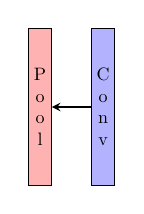
\begin{tikzpicture}[baseline=-0pt]
\filldraw[fill=blue!30!white] (0.8,-1) rectangle (0.8+0.3,1); 
\node[align=center,scale = 0.65] at (0.8+0.15,0)  {C \\ o \\ n \\ v};
\draw[-stealth]  (0.8,0) -- (0+0.3,0);
\filldraw[fill=red!30!white] (0,-1) rectangle (0+0.3,1); 
\node[align=center,scale = 0.65] at (0+0.15,0) {P \\ o \\ o \\ l};
\end{tikzpicture}
\caption{Backpropagate from conv to pool.}
\end{center}
\end{figure}
We show in appendix \ref{sec:appenderrorrate} that this induces the following error rate
\begin{align}
\delta^{(t)(\nu)}_{flm}&=
%
\sum^{F_{\nu+1}-1}_{f'=0}\sum^{R_C-1}_{j=0}\sum^{R_C-1}_{k=0}
%
\Theta^{(o)f}_{f'\,j\,k}\delta_{f\,\frac{l+P-j}{S_C}+P\,\frac{m+P-k}{S_C}+P}^{(t)(\nu+1)}\;.
\end{align}

\subsection{Weight update}

For the weight updates, we will also consider separately the weights between  fc  to fc layer, fc to pool, conv to conv, conv to pool and conv to input.

\subsubsection{Weight update from fc to fc}

For the two layer interactions

\begin{figure}[H]
\begin{center}
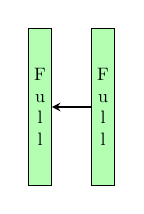
\begin{tikzpicture}[baseline=-0pt]
\filldraw[fill=green!30!white] (0.8,-1) rectangle (0.8+0.3,1); 
\node[align=center,scale = 0.65] at (0.8+0.15,0) {F \\ u \\ l \\ l};
\draw[-stealth]  (0.8,0) -- (0+0.3,0);
\filldraw[fill=green!30!white] (0,-1) rectangle (0+0.3,1); 
\node[align=center,scale = 0.65] at (0+0.15,0) {F \\ u \\ l \\ l};
\end{tikzpicture}
\caption{Weight update between two fc layers.}
\end{center}
\end{figure}

We have the weight update that reads
\begin{align}
\Delta^{\Theta(o)f}_{f'}&=\sum_{t=0}^{T_{{\rm mb}}-1} y^{(t)(n)}_{f'}\delta^{(t)(\nu)}_f
\end{align}

\subsubsection{Weight update from fc to pool}



For the two layer interactions

\begin{figure}[H]
\begin{center}
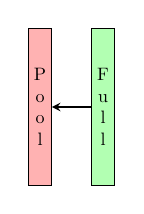
\begin{tikzpicture}[baseline=-0pt]
\filldraw[fill=green!30!white] (0.8,-1) rectangle (0.8+0.3,1); 
\node[align=center,scale = 0.65] at (0.8+0.15,0) {F \\ u \\ l \\ l};
\draw[-stealth]  (0.8,0) -- (0+0.3,0);
\filldraw[fill=red!30!white] (0,-1) rectangle (0+0.3,1); 
\node[align=center,scale = 0.65] at (0+0.15,0) {P \\ o \\ o \\ l};
\end{tikzpicture}
\caption{Weight update between a fc layer and a pool layer.}
\end{center}
\end{figure}

We have the weight update that reads
\begin{align}
\Delta^{\Theta(o)f}_{f'jk}&=\sum_{t=0}^{T_{{\rm mb}}-1} h^{(t)(\nu)}_{f'j+Pk+P}\delta^{(t)(\nu)}_f
\end{align}

\subsubsection{Weight update from conv to conv}

For the two layer interactions

\begin{figure}[H]
\begin{center}
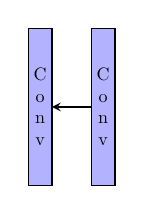
\begin{tikzpicture}[baseline=-0pt]
\filldraw[fill=blue!30!white] (0.8,-1) rectangle (0.8+0.3,1); 
\node[align=center,scale = 0.65] at (0.8+0.15,0)  {C \\ o \\ n \\ v};
\draw[-stealth]  (0.8,0) -- (0+0.3,0);
\filldraw[fill=blue!30!white] (0,-1) rectangle (0+0.3,1); 
\node[align=center,scale = 0.65] at (0+0.15,0) {C \\ o \\ n \\ v};
\end{tikzpicture}
\caption{Weight update between two conv layers.}
\end{center}
\end{figure}

We have the weight update that reads
\begin{align}
\Delta^{\Theta(o)f}_{f'jk}&=\sum_{t=0}^{T_{{\rm mb}}-1}\sum^{T_{\nu+1}-1}_{l=0}\sum^{N_{\nu+1}-1}_{m=0}
%
y^{(t)(n)}_{f'\,l+j\,m+k}\delta_{f\,l+P\,m+P}^{(t)(\nu)}
\end{align}

\subsubsection{Weight update from conv to pool and conv to input}

For the two layer interactions

\begin{figure}[H]
\begin{center}
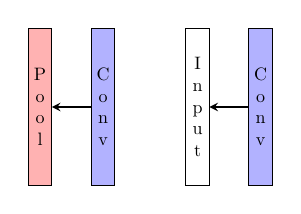
\begin{tikzpicture}[baseline=-0pt]
\filldraw[fill=blue!30!white] (0.8,-1) rectangle (0.8+0.3,1); 
\node[align=center,scale = 0.65] at (0.8+0.15,0)  {C \\ o \\ n \\ v};
\draw[-stealth]  (0.8,0) -- (0+0.3,0);
\filldraw[fill=red!30!white] (0,-1) rectangle (0+0.3,1); 
\node[align=center,scale = 0.65] at (0+0.15,0) {P \\ o \\ o \\ l};
%
\filldraw[fill=blue!30!white] (2.8,-1) rectangle (2.8+0.3,1); 
\node[align=center,scale = 0.65] at (2.8+0.15,0)  {C \\ o \\ n \\ v};
\draw[-stealth]  (2.8,0) -- (2+0.3,0);
\draw (2,-1) rectangle (2+0.3,1); 
\node[align=center,scale = 0.65] at (2+0.15,0) {I \\ n \\ p \\ u \\ t};
\end{tikzpicture}
\caption{Weight update between a conv and a pool layer, as well as between a conv and the input layer.}
\end{center}
\end{figure}
\begin{align}
\Delta^{\Theta(o)f}_{f'jk}&=\sum_{t=0}^{T_{{\rm mb}}-1}\sum^{T_{\nu+1}-1}_{l=0}\sum^{N_{\nu+1}-1}_{m=0}
%
h^{(t)(\nu)}_{f'\,l+j\,m+k}\delta_{f\,l+P\,m+P}^{(t)(\nu)}
\end{align}


\subsection{Coefficient update}


For the Coefficient updates, we will also consider separately the weights between  fc to fc layer, fc to pool, cont to pool and conv to conv.

\subsubsection{Coefficient update from fc to fc}

For the two layer interactions

\begin{figure}[H]
\begin{center}
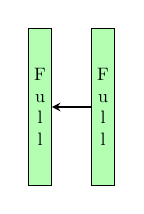
\begin{tikzpicture}[baseline=-0pt]
\filldraw[fill=green!30!white] (0.8,-1) rectangle (0.8+0.3,1); 
\node[align=center,scale = 0.65] at (0.8+0.15,0) {F \\ u \\ l \\ l};
\draw[-stealth]  (0.8,0) -- (0+0.3,0);
\filldraw[fill=green!30!white] (0,-1) rectangle (0+0.3,1); 
\node[align=center,scale = 0.65] at (0+0.15,0) {F \\ u \\ l \\ l};
\end{tikzpicture}
\caption{Coefficient update between two fc layers.}
\end{center}
\end{figure}

We have

\begin{align}
\Delta_f^{\gamma(n)}&=\sum_{t=0}^{T_{{\rm mb}}-1}\sum_{f'=0}^{F_{\nu+1}-1}
%
\Theta^{(o)f'}_{f}\tilde{h}^{(t)(n)}_{f}\delta^{(t)(\nu)}_{f'}\;,\notag\\
%
\Delta_f^{\beta(n)}&=
%
\sum_{t=0}^{T_{{\rm mb}}-1}\sum_{f'=0}^{F_{\nu+1}-1}\Theta^{(o)f'}_{f}\delta^{(t)(\nu)}_{f'}\;,
\end{align}

\subsubsection{Coefficient update from fc to pool and conv to pool}

For the two layer interactions

\begin{figure}[H]
\begin{center}
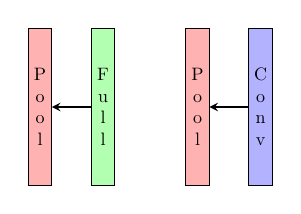
\begin{tikzpicture}[baseline=-0pt]
\filldraw[fill=green!30!white] (0.8,-1) rectangle (0.8+0.3,1); 
\node[align=center,scale = 0.65] at (0.8+0.15,0) {F \\ u \\ l \\ l};
\draw[-stealth]  (0.8,0) -- (0+0.3,0);
\filldraw[fill=red!30!white] (0,-1) rectangle (0+0.3,1); 
\node[align=center,scale = 0.65] at (0+0.15,0) {P \\ o \\ o \\ l};
%
\filldraw[fill=blue!30!white] (2.8,-1) rectangle (2.8+0.3,1); 
\node[align=center,scale = 0.65] at (2.8+0.15,0)  {C \\ o \\ n \\ v};
\draw[-stealth]  (2.8,0) -- (2+0.3,0);
\filldraw[fill=red!30!white] (2,-1) rectangle (2+0.3,1); 
\node[align=center,scale = 0.65] at (2+0.15,0) {P \\ o \\ o \\ l};
\end{tikzpicture}
\caption{Coefficient update between a fc layer and a pool as well as a conv and a pool layer.}
\end{center}
\end{figure}

\begin{align}
\Delta_f^{\gamma(n)}&=
%
\sum_{t=0}^{T_{{\rm mb}}-1}\sum_{l=0}^{N_{\nu+1}-1}\sum_{m=0}^{T_{\nu+1}-1}
%
\tilde{h}_{f\,S_P l+j_{flm}^{(t)(p)}+P\,S_Pm+k_{flm}^{(t)(p)}+P}^{(t)(n)}\delta^{(t)(\nu)}_{flm}\;,\notag\\
%
\Delta_f^{\beta(n)}&=
%
\sum_{t=0}^{T_{{\rm mb}}-1}\sum_{l=0}^{N_{\nu+1}-1}\sum_{m=0}^{T_{\nu+1}-1}\delta^{(t)(\nu)}_{flm}\;,
\end{align}


\subsubsection{Coefficient update from conv to conv}

For the two layer interactions

\begin{figure}[H]
\begin{center}
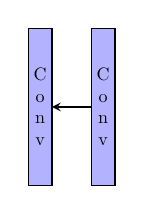
\begin{tikzpicture}[baseline=-0pt]
\filldraw[fill=blue!30!white] (0.8,-1) rectangle (0.8+0.3,1); 
\node[align=center,scale = 0.65] at (0.8+0.15,0)  {C \\ o \\ n \\ v};
\draw[-stealth]  (0.8,0) -- (0+0.3,0);
\filldraw[fill=blue!30!white] (0,-1) rectangle (0+0.3,1); 
\node[align=center,scale = 0.65] at (0+0.15,0) {C \\ o \\ n \\ v};
\end{tikzpicture}
\caption{Coefficient update between two conv layers.}
\end{center}
\end{figure}

We have


\begin{align}
\Delta_f^{\gamma(n)}&=
%
\sum_{t=0}^{T_{{\rm mb}}-1}\sum_{f'=0}^{F_{\nu+1}-1}\sum_{l=0}^{N_{\nu+1}-1}\sum_{m=0}^{T_{\nu+1}-1}
%
\sum_{j=0}^{R_C-1}\sum_{k=0}^{R_C-1}\Theta^{(o)f'}_{fjk}
%
\tilde{h}^{(t)(n)}_{fl+j\,m+k}\delta^{(t)(\nu)}_{f'\,l+P\,m+P}\;,\notag\\
%
\Delta_f^{\beta(n)}&=
%
\sum_{t=0}^{T_{{\rm mb}}-1}\sum_{f'=0}^{F_{\nu+1}-1}\sum_{l=0}^{N_{\nu+1}-1}\sum_{m=0}^{T_{\nu+1}-1}
%
\sum_{j=0}^{R_C-1}\sum_{k=0}^{R_C-1}\Theta^{(o)f'}_{fjk}\delta^{(t)(\nu)}_{f'\,l+P\,m+P}\;.
\end{align}

Let us now demonstrate all these formulas! 

\begin{subappendices}
\section{Backprop through BatchNorm} \label{sec:appenbatchnorm-vgg}


For Backpropagation, we will need 
\begin{align}
\frac{\partial y^{(t')(n)}_{f'\,l'\,m'}}{\partial h_{f\,l\,m}^{(t)(\nu)}}&=
%
\gamma^{(n)}_f\frac{\partial \tilde{h}_{f'\,l'\,m'}^{(t')(n)}}{\partial h_{f\,l\,m}^{(t)(\nu)}}\;.
\end{align}
Since
\begin{align}
\frac{\partial h^{(t')(\nu)}_{f'\,l'\,m'}}{\partial h_{f\,l\,m}^{(t)(\nu)}}&=\delta^{t'}_t\delta^{f'}_f
%
\delta^{l'}_l\delta^{m'}_m\;,&
%
\frac{\partial \hat{h}_{f'}^{(n)}}{\partial h_{f\,l\,m}^{(t)(\nu)}}&=\frac{\delta^{f'}_f}{T_{{\rm mb}}N_nT_n}\:;
\end{align}
and
\begin{align}
\frac{\partial \left(\hat{\sigma}_{f'}^{(n)}\right)^2}{\partial h_{f\,l\,m}^{(t)(\nu)}}&=
%
\frac{2\delta^{f'}_f}{T_{{\rm mb}}N_nT_n}\left(h_{f\,l\,m}^{(t)(\nu)}-\hat{h}_{f}^{(n)}\right)\;,
\end{align}
we get
\begin{align}
\frac{\partial \tilde{h}_{f'\,l'\,m'}^{(t')(n)}}{\partial h_{f\,l\,m}^{(t)(\nu)}}&=
%
\frac{\delta^{f'}_f}{T_{{\rm mb}}N_nT_n}\left[\frac{T_{{\rm mb}}N_nT_n\delta^{t'}_t
%
\delta^{l'}_l\delta^{m'}_m-1}
%
{\left(\left(\hat{\sigma}_{f}^{(n)}\right)^2+\epsilon\right)^\frac12}-
%
\frac{\left(h_{f\,l'\,m'}^{(t')(\nu)}-\hat{h}_{f}^{(n)}\right)\left(h_{f\,l\,m}^{(t)(\nu)}-\hat{h}_{f}^{(n)}\right)}
%
{\left(\left(\hat{\sigma}_{f}^{(n)}\right)^2+\epsilon\right)^\frac32}\right]\notag\\
%
&=\frac{\delta^{f'}_f}{\left(\left(\hat{\sigma}_{f}^{(n)}\right)^2+\epsilon\right)^\frac12}
%
\left[\delta^{t'}_t\delta^{l'}_l\delta^{m'}_m-
%
\frac{1+\tilde{h}_{f\,l'\,m'}^{(t')(n)}\tilde{h}_{f\,l\,m}^{(t)(n)}}{T_{{\rm mb}}N_nT_n}\right]\;.
\end{align}
To ease the notation we will denote
\begin{align}
\tilde{\gamma}^{(n)}_f&=
%
\frac{\gamma^{(n)}_f}{\left(\left(\hat{\sigma}_{f}^{(n)}\right)^2+\epsilon\right)^\frac12}\;.
\end{align}
%
%
%
so that
\begin{align}
\delta^f_{f'}J^{(tt')(n)}_{f\,l\,m\,l'\,m'}&=
%
\frac{\partial y_{f'\,l'\,m'}^{(t')(n)}}{\partial h_{f\,l\,m}^{(t)(\nu)}}=
%
\tilde{\gamma}^{(n)}_f \delta^{f'}_f\left[\delta^{t'}_t\delta^{l'}_l\delta^{m'}_m-
%
\frac{1+\tilde{h}_{f\,l'\,m'}^{(t')(n)}\tilde{h}_{f\,l\,m}^{(t)(n)}}{T_{{\rm mb}}N_nT_n}\right]\;.
\end{align}

\section{Error rate updates: details} \label{sec:appenderrorrate}

We have for backpropagation from fc to pool
\begin{align}
\delta^{(t)(\nu)}_{flm}&= \frac{\partial }{\partial  a_{flm}^{(t)(\nu)}}J^{(t)}(\Theta)=
%
\sum_{t'=0}^{T_{{\rm mb}}-1}\sum_{f'=0}^{F_{\nu+1}-1}
%
 \frac{\partial  a_{f'}^{(t')(\nu+1)}}{\partial  a_{flm}^{(t)(\nu)}} \delta^{(t')(\nu+1)}_{f'}\notag\\
%
&=\sum_{t'=0}^{T_{{\rm mb}}-1}\sum_{f'=0}^{F_{\nu+1}-1}\sum^{F_\nu-1}_{f''=0}
%
\sum^{N_{\nu+1}}_{j=0}\sum^{T_{\nu+1}}_{k=0}\Theta^{(o)f'}_{f''\,j\,k}
%
\frac{\partial h^{(t)(\nu+1)}_{f''j+Pk+P} }{\partial  h_{fl+Pm+P}^{(t)(\nu+1)}} \delta^{(t')(\nu+1)}_{f'}\notag\\
%
&=\sum_{f'=0}^{F_{\nu+1}-1}\Theta^{(o)f'}_{f\,l\,m} \delta^{(t)(\nu+1)}_{f'}\;,
\end{align}

For backpropagation from pool to conv

\begin{align}
\delta^{(t)(\nu)}_{fl+Pm+P}&=
%
\sum_{t'=0}^{T_{{\rm mb}}-1}\sum^{F_{\nu+1}-1}_{f'=0}\sum^{N_{\nu+1}-1}_{l'=0}\sum^{T_{\nu+1}-1}_{m'=0}
%
\frac{\partial a_{f'l'm'}^{(t')(\nu+1)}}{\partial a_{f\,l\,m}^{(t)(\nu)}}
%
\delta_{f'l'm'}^{(t')(\nu+1)}
%
=\notag\\
%
&=\sum_{t'=0}^{T_{{\rm mb}}-1}\sum^{F_{\nu+1}-1}_{f'=0}\sum^{N_{\nu+1}-1}_{l'=0}\sum^{T_{\nu+1}-1}_{m'=0}
%
\frac{\partial y_{f'\,S_P l'+j_{f'l'm'}^{(t')(p)}+P\,S_Pm'+k_{f'l'm'}^{(t')(p)}+P}^{(t')(n)}}{\partial h_{f\,l+P\,m+P}^{(t)(\nu+1)}}
%
g'\left(a_{f\,l\,m}^{(t)(\nu)}\right)\delta_{f'l'm'}^{(t')(\nu+1)}\notag\\
%
&=\tilde{\gamma}^{(n)}_fg'\left(a_{f\,l\,m}^{(t)(\nu)}\right)
%
\sum_{t'=0}^{T_{{\rm mb}}-1}\sum^{N_{\nu+1}-1}_{l'=0}\sum^{T_{\nu+1}-1}_{m'=0}\delta_{fl'm'}^{(t')(\nu+1)}\notag\\
%
&\left[\delta^{t'}_t\delta^{S_P l'+j_{t'fl'm'}^{(p)}}_l\delta^{S_Pm'+k_{t'fl'm'}^{(p)}}_m-
%
\frac{1+\tilde{h}_{f\,S_P l'+j_{fl'm'}^{(t')(p)}+P\,S_Pm'+k_{fl'm'}^{(t')(p)}+P}^{(t')(n)}\tilde{h}_{f\,l+P\,m+P}^{(t)(n)}}{T_{{\rm mb}}N_{n}T_{n}}\right]\notag\\
%
&=g'\left(a_{f\,l\,m}^{(t)(\nu)}\right)\sum_{t'=0}^{T_{{\rm mb}}-1}\sum^{N_{\nu+1}-1}_{l'=0}
%
\sum^{T_{\nu+1}-1}_{m'=0}\delta_{fl'm'}^{(t')(\nu+1)}\notag\\
%
&\times J^{(tt')(n)}_{f\,S_P l'+j_{fl'm'}^{(t')(p)}+P\,S_Pm'+k_{fl'm'}^{(t')(p)}+P\,l+P\,m+P}
\end{align}

For backpropagation from conv to conv

\begin{align}
\delta^{(t)(\nu)}_{fl+Pm+P}&=
%
\sum_{t'=0}^{T_{{\rm mb}}-1}\sum^{F_{\nu+1}-1}_{f'=0}\sum^{N_{\nu+1}-1}_{l'=0}\sum^{T_{\nu+1}-1}_{m'=0}
%
\frac{\partial a_{f'l'm'}^{(t')(\nu+1)}}{\partial a_{f\,l\,m}^{(t)(\nu)}}
%
\delta_{f'l'+Pm'+P}^{(t')(\nu+1)}\notag\\
%
&=\sum_{t'=0}^{T_{{\rm mb}}-1}\sum^{F_{\nu+1}-1}_{f'=0}\sum^{N_{\nu+1}-1}_{l'=0}\sum^{T_{\nu+1}-1}_{m'=0}
%
\sum^{F_{\nu+1}-1}_{f''=0}\sum^{R_C-1}_{j=0}\sum^{R_C-1}_{k=0}
%
\Theta^{(o)f'}_{f''\,j\,k}\notag\\
%
&\times\frac{\partial  y^{(t')(n)}_{f''\,l'+j\,m'+k}}{\partial h_{f\,l+P\,m+P}^{(t)(\nu+1)}}
%
g'\left(a_{f\,l\,m}^{(t)(\nu)}\right)\delta_{f'l'+Pm'+P}^{(t')(\nu+1)}\;,
\end{align}
so
\begin{align}
\delta^{(t)(\nu)}_{fl+Pm+P}&=\tilde{\gamma}^{(n)}_fg'\left(a_{f\,l\,m}^{(t)(\nu)}\right)
%
\sum_{t'=0}^{T_{{\rm mb}}-1}\sum^{F_{\nu+1}-1}_{f'=0}\sum^{N_{\nu+1}-1}_{l'=0}\sum^{T_{\nu+1}-1}_{m'=0}
%
\sum^{R_C-1}_{j=0}\sum^{R_C-1}_{k=0}\Theta^{(o)f'}_{f\,j\,k}\delta_{f'l'+Pm'+P}^{(t')(\nu+1)}\notag\\
%
&\times \left[\delta^{t'}_t\delta^{ l'+j}_{l+P}\delta^{m'+k}_{m+P}-
%
\frac{1+\tilde{h}_{f\, l'+j\,m'+k}^{(t')(n)}\tilde{h}_{f\,l+P\,m+P}^{(t)(n)}}{T_{{\rm mb}}N_nT_n}\right]\notag\\
%
&=g'\left(a_{f\,l\,m}^{(t)(\nu)}\right)
%
\sum_{t'=0}^{T_{{\rm mb}}-1}\sum^{F_{\nu+1}-1}_{f'=0}\sum^{N_{\nu+1}-1}_{l'=0}\sum^{T_{\nu+1}-1}_{m'=0}
%
\sum^{R_C-1}_{j=0}\sum^{R_C-1}_{k=0}\delta_{f'l'+Pm'+P}^{(t')(\nu+1)}\notag\\
%
&\times \Theta^{(o)f'}_{f\,j\,k} J^{(tt')(n)}_{f\, l'+j\,m'+k\,l+P\,m+P}\;,
\end{align}

and for backpropagation from conv to pool (taking the stride equal to 1 to simplify the derivation)

\begin{align}
\delta^{(t)(\nu)}_{flm}&=
%
\sum_{t'=0}^{T_{{\rm mb}}-1}\sum^{F_{\nu+1}-1}_{f'=0}\sum^{N_{\nu+1}-1}_{l'=0}\sum^{T_{\nu+1}-1}_{m'=0}
%
\frac{\partial a_{f'l'm'}^{(t')(\nu+1)}}{\partial a_{f\,l\,m}^{(t)(\nu)}}
%
\delta_{f'l'+Pm'+P}^{(t')(\nu+1)}\notag\\
%
&=\sum_{t'=0}^{T_{{\rm mb}}-1}\sum^{F_{\nu+1}-1}_{f'=0}\sum^{N_{\nu+1}-1}_{l'=0}\sum^{T_{\nu+1}-1}_{m'=0}
%
\sum^{F_{\nu+1}-1}_{f''=0}\sum^{R_C-1}_{j=0}\sum^{R_C-1}_{k=0}
%
\Theta^{(o)f'}_{f''\,j\,k}
%
\frac{\partial  h^{(t')(\nu+1)}_{f''\,l'+j\,m'+k}}{\partial h_{f\,l+P\,m+P}^{(t)(\nu+1)}}
%
\delta_{f'l'+Pm'+P}^{(t')(\nu+1)}\notag\\
%
&=\sum^{F_{\nu+1}-1}_{f'=0}\sum^{R_C-1}_{j=0}\sum^{R_C-1}_{k=0}
%
\Theta^{(o)f'}_{f\,j\,k}\delta_{f'l+2P-j\,m+2P-k}^{(t)(\nu+1)}\;.
\end{align}

And so on and so forth.

\section{Weight update: details}
Fc to Fc
\begin{align}
\Delta^{\Theta(o)f}_{f'}&=\frac{1}{T_{{\rm mb}}}\sum_{t=0}^{T_{{\rm mb}}-1}
%
\sum^{F_{\nu+1}-1}_{f''=0}\sum^{F_\nu}_{f'''=0}\frac{\partial\Theta^{(o)f''}_{f'''}
%
}{\partial \Theta^{(o)f}_{f'}}y^{(t)(n)}_{f'''}\delta^{(t)(\nu)}_{f''}
%
=\sum_{t=0}^{T_{{\rm mb}}-1}\delta^{(t)(\nu)}_f y^{(t)(n)}_{f'}\;.
\end{align}
Fc to pool
\begin{align}
\Delta^{\Theta(o)f}_{f'jk}&=\frac{1}{T_{{\rm mb}}}\sum_{t=0}^{T_{{\rm mb}}-1}
%
\sum^{F_{\nu+1}-1}_{f''=0}\sum^{F_\nu}_{f'''=0}\sum^{N_{\nu+1}}_{j'=0}\sum^{T_{\nu+1}}_{k'=0}
%
\frac{\partial\Theta^{(13)f''}_{f'''j'k'}
%
}{\partial \Theta^{(o)f}_{f'jk}}h^{(t)(\nu)}_{f'''j'+Pk'+P}\delta^{(t)(\nu)}_{f''}\notag\\
%
&=\sum_{t=0}^{T_{{\rm mb}}-1}\delta^{(t)(\nu)}_f h^{(t)(\nu)}_{f'j+Pk+P}\;.
\end{align}
and for conv to conv
\begin{align}
\Delta^{\Theta(o)f}_{f'jk}&=\sum_{t=0}^{T_{{\rm mb}}-1}\sum^{F_{\nu+1}-1}_{f''=0}\sum^{T_{\nu+1}-1}_{l=0}\sum^{N_{\nu+1}-1}_{m=0}
%
\frac{\partial a_{f''\,l\,m}^{(t)(\nu)}}{\partial \Theta^{(o)f}_{f'\,j\,k}}
%
\delta_{f''\,l+P\,m+P}^{(t)(\nu)}\notag\\
%
&=\sum_{t=0}^{T_{{\rm mb}}-1}\sum^{F_{\nu+1}-1}_{f''=0}\sum^{T_{\nu+1}-1}_{l=0}\sum^{N_{\nu+1}-1}_{m=0}
%
\sum^{F_{\nu+1}-1}_{f'''=0}\sum^{R_C-1}_{j'=0}\sum^{R_C-1}_{k'=0}
%
\frac{\partial \Theta^{(o)f''}_{f'''\,j'\,k'}}{\partial \Theta^{(o)f}_{f'\,j\,k}}\notag\\
%
&\times y^{(t)(n)}_{f'''\,S_Cl+j'\,S_Cm+k'}
%
\delta_{f''\,l+P\,m+P}^{(t)(\nu)}\notag\\
%
&=\sum_{t=0}^{T_{{\rm mb}}-1}\sum^{T_{\nu+1}-1}_{l=0}\sum^{N_{\nu+1}-1}_{m=0}
%
y^{(t)(n)}_{f'\,S_Cl+j\,S_Cm+k}\delta_{f\,l+P\,m+P}^{(t)(\nu)}\;.
\end{align}
similarly for conv to pool and conv to input
\begin{align}
\Delta^{\Theta(o)f}_{f'jk}&=\sum_{t=0}^{T_{{\rm mb}}-1}\sum^{T_{\nu+1}-1}_{l=0}\sum^{N_{\nu+1}-1}_{m=0}
%
h^{(t)(\nu)}_{f'\,S_Cl+j\,S_Cm+k}\delta_{f\,l+P\,m+P}^{(t)(\nu)}\;.
\end{align}
%
%
\section{Coefficient update: details}
Fc to Fc
\begin{align}
\Delta_f^{\gamma(n)}&=\sum_{t=0}^{T_{{\rm mb}}-1}\sum_{f'=0}^{F_{\nu+1}-1}
%
\frac{\partial a^{(t)(\nu+1)}_{f'}}{\partial\gamma_f^{(n)}}\delta^{(t)(\nu+1)}_{f'}
%
=\sum_{t=0}^{T_{{\rm mb}}-1}\sum_{f'=0}^{F_{\nu+1}-1}
%
\Theta^{(o)f'}_{f}\tilde{h}^{(t)(n)}_{f}\delta^{(t)({\nu+1})}_{f'}\;,\\
%
\Delta_f^{\beta(n)}&=\sum_{t=0}^{T_{{\rm mb}}-1}\sum_{f'=0}^{F_{\nu+1}-1}
%
\frac{\partial a^{(t)(\nu+1)}_{f'}}{\partial\beta_f^{(n)}}\delta^{(t)(\nu+1)}_{f'}
%
=\sum_{t=0}^{T_{{\rm mb}}-1}\sum_{f'=0}^{F_{\nu+1}-1}\Theta^{(o)f'}_{f}\delta^{(t)(\nu+1)}_{f'}\;,
\end{align}
fc to pool and conv to pool
\begin{align}
\Delta_f^{\gamma(n)}&=
%
\sum_{t=0}^{T_{{\rm mb}}-1}\sum_{l=0}^{N_{\nu+1}-1}\sum_{m=0}^{T_{\nu+1}-1}
%
\tilde{h}_{f\,S_P l+j_{flm}^{(t)(p)}+P\,S_Pm+k_{flm}^{(t)(p)}+P}^{(t)(n)}\delta^{(t)(\nu+1)}_{flm}\\
%
\Delta_f^{\beta(n)}&=
%
\sum_{t=0}^{T_{{\rm mb}}-1}\sum_{l=0}^{N_{\nu+1}-1}\sum_{m=0}^{T_{\nu+1}-1}\delta^{(t)(\nu+1)}_{flm}\;,
\end{align}
conv to conv
\begin{align}
\Delta_f^{\gamma(n)}&=
%
\sum_{t=0}^{T_{{\rm mb}}-1}\sum_{f'=0}^{F_{\nu+1}-1}\sum_{l=0}^{N_{\nu+1}-1}\sum_{m=0}^{T_{\nu+1}-1}
%
\frac{a^{(t)(\nu+1)}_{f'lm}}{\partial \gamma_f^{(n)}}\delta^{(t)(\nu+1)}_{f'lm}\\
%
&=\sum_{t=0}^{T_{{\rm mb}}-1}\sum_{f'=0}^{F_{\nu+1}-1}\sum_{l=0}^{N_{\nu+1}-1}\sum_{m=0}^{T_{\nu+1}-1}
%
\sum_{j=0}^{R_C-1}\sum_{k=0}^{R_C-1}\Theta^{(o)f'}_{fjk}
%
\tilde{h}^{(t)(n)}_{fl+j\,m+k}\delta^{(t)(\nu+1)}_{f'lm}\\
%
\Delta_f^{\beta(n)}&=
%
\sum_{t=0}^{T_{{\rm mb}}-1}\sum_{f'=0}^{F_{\nu+1}-1}\sum_{l=0}^{N_{\nu+1}-1}\sum_{m=0}^{T_{\nu+1}-1}
%
\sum_{j=0}^{R_C-1}\sum_{k=0}^{R_C-1}\Theta^{(o)f'}_{fjk}\delta^{(t)(\nu+1)}_{f'lm}\;,
\end{align}

\section{Practical Simplification} \label{sec:pracsimpl}

When implementing a CNN, it turns out that some of the error rate computation can be very costly (in term of execution time) if naively encoded. In this section, we sketch some improvement that can be performed on the pool to conv, conv to conv  error rate implementation, as well as ones on coefficient updates.

\subsection{pool to conv Simplification}

Let us expand the batch normalization term of the pool to conv error rate to see how we can simplify it (calling the pooling the $p$'th one)
\begin{align}
\delta^{(t)(\nu)}_{flm}&=\tilde{\gamma}^{(n)}_fg'\left(a_{f\,l\,m}^{(t)(\nu)}\right)
%
\sum_{t'=0}^{T_{{\rm mb}}-1}\sum^{N_{\nu+1}-1}_{l'=0}\sum^{T_{\nu+1}-1}_{m'=0}\delta_{fl'm'}^{(t')(\nu+1)}\notag\\
%
&\left[\delta^{t'}_t\delta^{S_P l'+j_{t'fl'm'}^{(p)}}_l\delta^{S_Pm'+k_{t'fl'm'}^{(p)}}_m-
%
\frac{1+\tilde{h}_{f\,S_P l'+j_{fl'm'}^{(t')(p)}+P\,S_Pm'+k_{fl'm'}^{(t')(p)}+P}^{(t')(n)}\tilde{h}_{f\,l+P\,m+P}^{(t)(n)}}{T_{{\rm mb}}N_nT_n}\right]\;.
\end{align}
Numerically, this implies that for each $t,f,l,m$ one needs to perform 3 loops (on $t',l',m'$), hence a 7 loop process. This can be reduced to 4 at most in the following way. Defining
\begin{align}
\mu_f^{(1)}&=
%
\sum_{t'=0}^{T_{{\rm mb}}-1}\sum^{N_{\nu+1}-1}_{l'=0}\sum^{T_{\nu+1}-1}_{m'=0}
%
\delta_{fl'm'}^{(t')(\nu+1)}\;,
\end{align}
and
\begin{align}
\mu_f^{(2)}&=
%
\sum_{t'=0}^{T_{{\rm mb}}-1}\sum^{N_{\nu+1}-1}_{l'=0}\sum^{T_{\nu+1}-1}_{m'=0}\delta_{fl'm'}^{(t')(\nu+1)}
%
\tilde{h}_{f\,S_P l'+j_{fl'm'}^{(t')(p)}+P\,S_Pm'+k_{fl'm'}^{(t')(p)}+P}^{(t')(n)}\;,
\end{align}
we have introduced two new variables that can be computed in four loops, but three of them are independent of the ones needed to compute $\delta^{(t)(\nu)}_{flm}$. For the last term, the $\delta$ functions "kill" 3 loops and we are left with
\begin{align}
\delta^{(t)(\nu)}_{flm}=\tilde{\gamma}^{(n)}_fg'\left(a_{f\,l\,m}^{(t)(\nu)}\right)&\left\{
%
\sum^{N_{\nu+1}-1}_{l'=0}\sum^{T_{\nu+1}-1}_{m'=0}\delta_{fl'm'}^{(t')(\nu+1)}
%
\delta^{S_P l'+j_{t'fl'm'}^{(p)}}_l\delta^{S_Pm'+k_{t'fl'm'}^{(p)}}_m\right.\notag\\
%
&-\left.
%
\frac{\mu_f^{(1)}+\mu_f^{(2)}\tilde{h}_{f\,l+P\,m+P}^{(t)(n)}}{T_{{\rm mb}}N_nT_n}\right\}\;,
\end{align}
which requires only 4 loops to be computed.

\subsection{Convolution Simplification}

Let us expand the batch normalization term of the conv to conv error rate to see how we can simplify it
\begin{align}
\delta^{(t)(\nu)}_{flm}&=\tilde{\gamma}^{(n)}_fg'\left(a_{f\,l\,m}^{(t)(i\nu)}\right)
%
\sum_{t'=0}^{T_{{\rm mb}}-1}\sum^{F_{\nu+1}-1}_{f'=0}\sum^{N_{\nu+1}-1}_{l'=0}\sum^{T_{\nu+1}-1}_{m'=0}
%
\sum^{R_C-1}_{j=0}\sum^{R_C-1}_{k=0}\Theta^{(o)f'}_{f\,j\,k}\delta_{f'l'm'}^{(t')(\nu+1)}\notag\\
%
&\left[\delta^{t'}_t\delta^{ l'+j}_{l+P}\delta^{m'+k}_{m+P}-
%
\frac{1+\tilde{h}_{f\, l'+j\,m'+k}^{(t')(n)}\tilde{h}_{f\,l+P\,m+P}^{(t)(n)}}{T_{{\rm mb}}N_nT_n}\right]\;.
\end{align}
If left untouched, one now needs 10 loops (on $t,f,l,m$ and $t',f',l',m',j,k$) to compute $\delta^{(t)(\nu)}_{flm}$ ! This can be reduced to 7 loops at most in the following way. First, we define
\begin{align}
\lambda^{(t)(1)}_{flm}&=\sum^{F_{\nu+1}-1}_{f'=0}\sum^{R_C-1}_{j=0}\sum^{R_C-1}_{k=0}
%
\Theta^{(o)f'}_{f\,j\,k}\delta_{f'l+P-j\,m+P-k}^{(t')(\nu+1)}\;,
\end{align}
which is a convolution operation on a shifted index $\delta^{(\nu+1)}$. This is second most expensive operation, but libraries are optimized for this and it implies two of the smallest loops (those on $R_C$). Then we compute (four loops each)
\begin{align}
\lambda^{(2)}_{ff'}&=\sum^{R_C-1}_{j=0}\sum^{R_C-1}_{k=0}\Theta^{(o)f'}_{f\,j\,k}\;,&
%
\lambda^{(3)}_{f'}&=\sum_{t'=0}^{T_{{\rm mb}}-1}\sum^{N_{\nu+1}-1}_{l'=0}\sum^{T_{\nu+1}-1}_{m'=0}
%
\delta_{f'l'm'}^{(t')(\nu+1)}\;,
\end{align}
and (2 loops)
\begin{align}
\lambda^{(4)}_{f}&=\sum^{F_{\nu+1}-1}_{f'=0}\lambda^{(2)}_{ff'}\lambda^{(3)}_{f'}\;.
\end{align}
Finally, we compute
\begin{align}
\lambda^{(5)}_{ff'jk}&=\sum_{t'=0}^{T_{{\rm mb}}-1}\sum^{N_{\nu+1}-1}_{l'=0}\sum^{T_{\nu+1}-1}_{m'=0}
%
\delta_{f'l'm'}^{(t')(\nu+1)}\tilde{h}_{f\, l'+j\,m'+k}^{(t')(n)}\;,\\
%
\lambda^{(6)}_{f}&=\sum^{F_{\nu+1}-1}_{f'=0}\sum^{R_C-1}_{j=0}\sum^{R_C-1}_{k=0}
%
\Theta^{(o)f'}_{f\,j\,k}\lambda^{(5)}_{ff'jk}\;.
\end{align}
$\lambda^{(6)}_{f}$ only requires four loops, and $\lambda^{(5)}_{ff'jk}$ is the  most expensive operation. But it is also a convolution operation that implies two of the smallest loops (those on $R_C$). With all these newly introduced $\lambda$, we obtain
\begin{align}
\delta^{(t)(\nu)}_{flm}&=\tilde{\gamma}^{(n)}_fg'\left(a_{f\,l\,m}^{(t)(\nu)}\right)\left\{
%
\lambda^{(t)(1)}_{flm}-
%
\frac{\lambda^{(4)}_{f}+\lambda^{(6)}_{f}\tilde{h}_{f\,l+P\,m+P}^{(t)(n)}}{T_{{\rm mb}}N_nT_n}\right\}\;,
\end{align}
which only requires four loops to be computed.

\subsection{Coefficient Simplification}

To compute
\begin{align}
\Delta_f^{\gamma(n)}
%
&=\sum_{t=0}^{T_{{\rm mb}}-1}\sum_{f'=0}^{F_{\nu+1}-1}\sum_{l=0}^{N_{\nu+1}-1}\sum_{m=0}^{T_{\nu+1}-1}
%
\sum_{j=0}^{R_C-1}\sum_{k=0}^{R_C-1}\Theta^{(o)f'}_{fjk}
%
\tilde{h}^{(t)(n)}_{fl+j\,m+k}\delta^{(t)(\nu+1)}_{f'lm}\\
%
\Delta_f^{\beta(n)}&=
%
\sum_{t=0}^{T_{{\rm mb}}-1}\sum_{f'=0}^{F_{\nu+1}-1}\sum_{l=0}^{N_{\nu+1}-1}\sum_{m=0}^{T_{\nu+1}-1}
%
\sum_{j=0}^{R_C-1}\sum_{k=0}^{R_C-1}\Theta^{(o)f'}_{fjk}\delta^{(t)(\nu+1)}_{f'lm}\;,
\end{align}
we will first define
\begin{align}
\nu^{(1)}_{f'fjk}&=\sum_{t=0}^{T_{{\rm mb}}-1}\sum_{l=0}^{N_{\nu+1}-1}\sum_{m=0}^{T_{\nu+1}-1}
%
\tilde{h}^{(t)(n)}_{fl+j\,m+k}\delta^{(t)(\nu+1)}_{f'lm}\;,&
%
\nu^{(2)}_{f'}&=\sum_{t=0}^{T_{{\rm mb}}-1}\sum_{l=0}^{N_{\nu+1}-1}\sum_{m=0}^{T_{\nu+1}-1}
%
\delta^{(t)(\nu+1)}_{f'lm}\;,
\end{align}
so that
\begin{align}
\Delta_f^{\gamma(n)}&=\sum_{f'=0}^{F_{\nu+1}-1}\sum_{j=0}^{R_C-1}
%
\sum_{k=0}^{R_C-1}\nu^{(1)}_{f'fjk}\Theta^{(o)f'}_{fjk}\;\\
%
\Delta_f^{\beta(n)}&=
%
\sum_{f'=0}^{F_{\nu+1}-1}\sum_{j=0}^{R_C-1}\sum_{k=0}^{R_C-1}\nu^{(2)}_{f'}\Theta^{(o)f'}_{fjk}\;,
\end{align}


\section{Batchpropagation through a ResNet module}

For pedagogical reasons, we introduced the ResNet structure without "breaking" the conv layers. Nevertheless, a more standard choice is depicted in the following figure

\begin{figure}[H]
\begin{center}
\begin{tikzpicture}[baseline=-0pt]
\node at (0,0) {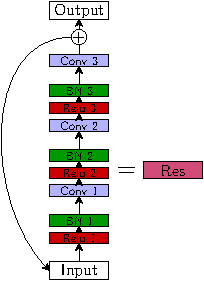
\includegraphics[scale=1]{Bottleneck_BN_backprop_2}};
\end{tikzpicture}
\caption{Batchpropagation through a ResNet module.}
\end{center}
\end{figure}

Batchpropagation through this ResNet module presents no particular difficulty. Indeed, the update rules imply the usual conv to conv backpropagation derived in the main part of this note. The only novelty is the error rate update of the input layer of the ResNet, as it now reads (assuming that the input of  this ResNet module is the output of another one)

\begin{align}
\delta^{(t)(\nu)}_{fl+Pm+P}&=
%
\sum_{t'=0}^{T_{{\rm mb}}-1}\sum^{F_{\nu+1}-1}_{f'=0}\sum^{N_{\nu+1}-1}_{l'=0}\sum^{T_{\nu+1}-1}_{m'=0}
%
\frac{\partial a_{f'l'm'}^{(t')(\nu+1)}}{\partial a_{f\,l\,m}^{(t)(\nu)}}
%
\delta_{f'l'+Pm'+P}^{(t')(\nu+1)}\notag\\
%
&+\sum_{t'=0}^{T_{{\rm mb}}-1}\sum^{F_{\nu+3}-1}_{f'=0}\sum^{N_{\nu+3}-1}_{l'=0}\sum^{T_{\nu+3}-1}_{m'=0}
%
\frac{\partial a_{f'l'm'}^{(t')(\nu+3)}}{\partial a_{f\,l\,m}^{(t)(\nu)}}
%
\delta_{f'l'+Pm'+P}^{(t')(\nu+3)}\notag\\
%
&=g'\left(a_{f\,l\,m}^{(t)(\nu)}\right)
%
\sum_{t'=0}^{T_{{\rm mb}}-1}\sum^{F_{\nu+1}-1}_{f'=0}\sum^{N_{\nu+1}-1}_{l'=0}\sum^{T_{\nu+1}-1}_{m'=0}
%
\sum^{R_C-1}_{j=0}\sum^{R_C-1}_{k=0}\delta_{f'l'+Pm'+P}^{(t')(\nu+1)}\notag\\
%
&\times \Theta^{(o)f'}_{f\,j\,k} J^{(tt')(n)}_{f\, l'+j\,m'+k\,l+P\,m+P}
%
+\delta_{fl+Pm+P}^{(t)(\nu+3)}\;.
\end{align}
This new term is what allows the error rate to flow smoothly from the output to the input in the ResNet CNN, as the additional connexion in a ResNet is like a skip path to the convolution chains. Let us mention in passing that some architecture connects every hidden layer to each others\cite{HuangGLZLW}.


\section{Convolution as a matrix multiplication}

Thanks to the simplifications introduced in appendix \ref{sec:pracsimpl}, we have reduced all convolution, pooling and tensor multiplication operations to at most 7 loops operations. Nevertheless, in high abstraction programming languages such as python, it is still way too much to be handled smoothly. But there exists additional tricks to "reduce" the dimension of the convolution operation, such as one has only to encode three for loops (2D matrix multiplication) at the end of the day. Let us begin our presentation of these tricks with a 2D convolution example

\subsection{2D Convolution}


\begin{figure}[H]
\begin{center}
\begin{tikzpicture}[baseline=-0pt]
\node at (0,0) {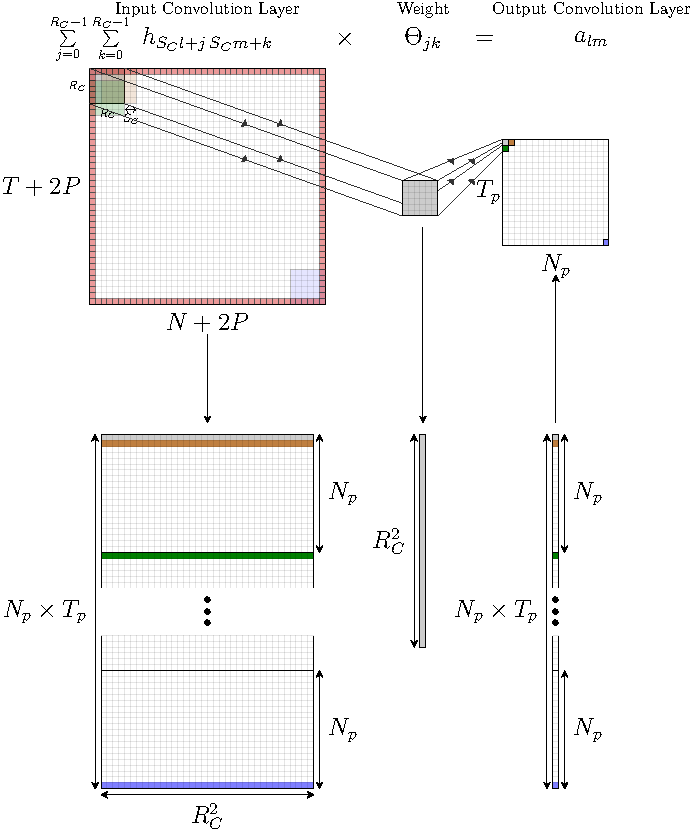
\includegraphics[scale=0.8]{conv_2d-crop}};
\end{tikzpicture}
\caption{\label{fig:2dconv}:2D convolution as a 2D matrix multiplication}
\end{center}
\end{figure}


A 2D convolution operation reads
\begin{align}
a_{lm}&=\sum_{j=0}^{R_C-1}\sum_{k=0}^{R_C-1}\Theta_{jk}h_{S_Cl+j\,S_Cm+k}\;.
\end{align}
and it involves 4 loops. The trick to reduce this operation to a 2D matrix multiplication is to redefine the $h$ matrix by looking at each $h$ indices are going to be multiplied by $\Theta$ for each value of $l$ and $m$. Then the associated $h$ values are stored into a $N_pT_p\times R_C^2$ matrix. Flattening out the $\Theta$ matrix, we are left with a matrix multiplication, the flattened $\Theta$ matrix being of size $R_C^2\times 1$. This is illustrated on figure \ref{fig:2dconv}

\subsection{4D Convolution}

\begin{figure}[H]
\begin{center}
\begin{tikzpicture}[baseline=-0pt]
\node at (0,0) {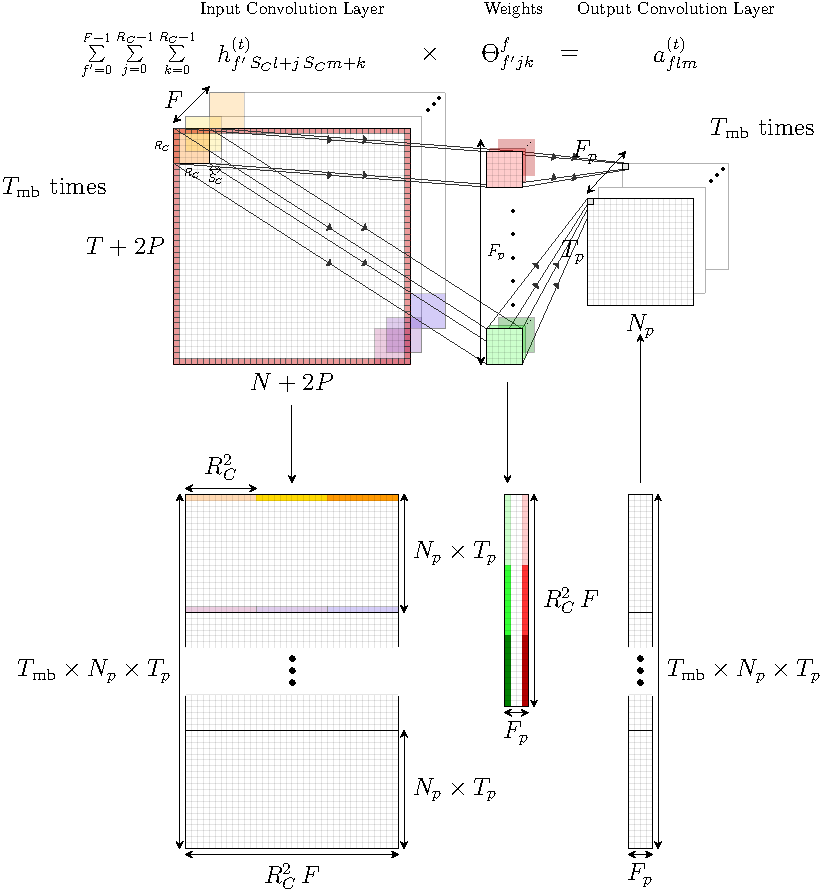
\includegraphics[scale=0.75]{conv_4d-crop}};
\end{tikzpicture}
\caption{\label{fig:4dconv}4D convolution as a 2D matrix multiplication}
\end{center}
\end{figure}



Following the same lines, the adding of the input and output feature maps as well as the batch size poses no particular conceptual difficulty, as illustrated on figure \ref{fig:4dconv}, corresponding to the 4D convolution
\begin{align}
a^{(t)}_{flm}&=
%
\sum_{f'=0}^{F_p-1}\sum_{j=0}^{R_C-1}\sum_{k=0}^{R_C-1}\Theta^f_{f'jk}h^{(t)}_{f'S_Cl+j\,S_Cm+k}\;.
\end{align}


\section{Pooling as a row matrix maximum}

\begin{figure}[H]
\begin{center}
\begin{tikzpicture}[baseline=-0pt]
\node at (0,0) {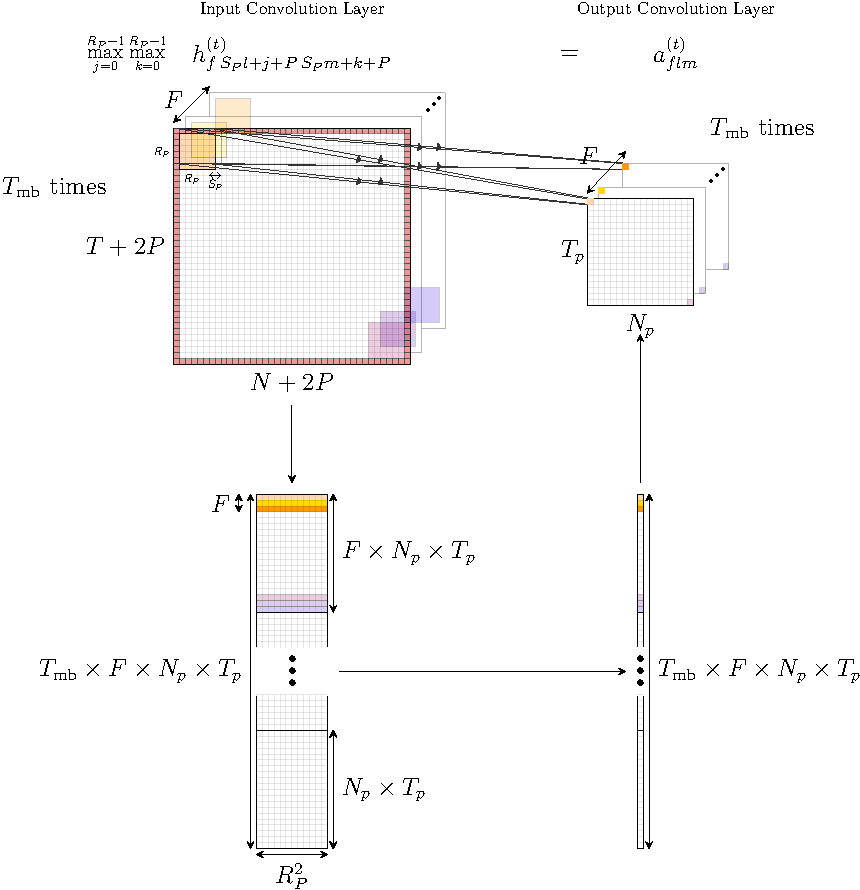
\includegraphics[scale=0.75]{pool_4d-crop}};
\end{tikzpicture}
\caption{\label{fig:4dpool}4D pooling as a 2D matrix multiplication}
\end{center}
\end{figure}

The pooling operation can also be simplified, seeing it as the maximum search on the rows of a flattened 2D matrix. This is illustrated on figure \ref{fig:4dpool}
\begin{align}
a^{(t)}_{flm}&=
%
\max_{j=0}^{R_P-1}\max_{k=0}^{R_P-1}h^{(t)}_{fS_Pl+j\,S_Pm+k}\;.
\end{align}
\end{subappendices}
